\documentclass[twoside]{book}

% Packages required by doxygen
\usepackage{fixltx2e}
\usepackage{calc}
\usepackage{doxygen}
\usepackage[export]{adjustbox} % also loads graphicx
\usepackage{graphicx}
\usepackage[utf8]{inputenc}
\usepackage{makeidx}
\usepackage{multicol}
\usepackage{multirow}
\PassOptionsToPackage{warn}{textcomp}
\usepackage{textcomp}
\usepackage[nointegrals]{wasysym}
\usepackage[table]{xcolor}

% Font selection
\usepackage[T1]{fontenc}
\usepackage[scaled=.90]{helvet}
\usepackage{courier}
\usepackage{amssymb}
\usepackage{sectsty}
\renewcommand{\familydefault}{\sfdefault}
\allsectionsfont{%
  \fontseries{bc}\selectfont%
  \color{darkgray}%
}
\renewcommand{\DoxyLabelFont}{%
  \fontseries{bc}\selectfont%
  \color{darkgray}%
}
\newcommand{\+}{\discretionary{\mbox{\scriptsize$\hookleftarrow$}}{}{}}

% Page & text layout
\usepackage{geometry}
\geometry{%
  a4paper,%
  top=2.5cm,%
  bottom=2.5cm,%
  left=2.5cm,%
  right=2.5cm%
}
\tolerance=750
\hfuzz=15pt
\hbadness=750
\setlength{\emergencystretch}{15pt}
\setlength{\parindent}{0cm}
\setlength{\parskip}{0.2cm}
\makeatletter
\renewcommand{\paragraph}{%
  \@startsection{paragraph}{4}{0ex}{-1.0ex}{1.0ex}{%
    \normalfont\normalsize\bfseries\SS@parafont%
  }%
}
\renewcommand{\subparagraph}{%
  \@startsection{subparagraph}{5}{0ex}{-1.0ex}{1.0ex}{%
    \normalfont\normalsize\bfseries\SS@subparafont%
  }%
}
\makeatother

% Headers & footers
\usepackage{fancyhdr}
\pagestyle{fancyplain}
\fancyhead[LE]{\fancyplain{}{\bfseries\thepage}}
\fancyhead[CE]{\fancyplain{}{}}
\fancyhead[RE]{\fancyplain{}{\bfseries\leftmark}}
\fancyhead[LO]{\fancyplain{}{\bfseries\rightmark}}
\fancyhead[CO]{\fancyplain{}{}}
\fancyhead[RO]{\fancyplain{}{\bfseries\thepage}}
\fancyfoot[LE]{\fancyplain{}{}}
\fancyfoot[CE]{\fancyplain{}{}}
\fancyfoot[RE]{\fancyplain{}{\bfseries\scriptsize Generated on Fri Jul 24 2015 18\+:38\+:59 for Gender\+\_\+\+Recognition by Doxygen }}
\fancyfoot[LO]{\fancyplain{}{\bfseries\scriptsize Generated on Fri Jul 24 2015 18\+:38\+:59 for Gender\+\_\+\+Recognition by Doxygen }}
\fancyfoot[CO]{\fancyplain{}{}}
\fancyfoot[RO]{\fancyplain{}{}}
\renewcommand{\footrulewidth}{0.4pt}
\renewcommand{\chaptermark}[1]{%
  \markboth{#1}{}%
}
\renewcommand{\sectionmark}[1]{%
  \markright{\thesection\ #1}%
}

% Indices & bibliography
\usepackage{natbib}
\usepackage[titles]{tocloft}
\setcounter{tocdepth}{3}
\setcounter{secnumdepth}{5}
\makeindex

% Hyperlinks (required, but should be loaded last)
\usepackage{ifpdf}
\ifpdf
  \usepackage[pdftex,pagebackref=true]{hyperref}
\else
  \usepackage[ps2pdf,pagebackref=true]{hyperref}
\fi
\hypersetup{%
  colorlinks=true,%
  linkcolor=blue,%
  citecolor=blue,%
  unicode%
}

% Custom commands
\newcommand{\clearemptydoublepage}{%
  \newpage{\pagestyle{empty}\cleardoublepage}%
}


%===== C O N T E N T S =====

\begin{document}

% Titlepage & ToC
\hypersetup{pageanchor=false,
             bookmarks=true,
             bookmarksnumbered=true,
             pdfencoding=unicode
            }
\pagenumbering{roman}
\begin{titlepage}
\vspace*{7cm}
\begin{center}%
{\Large Gender\+\_\+\+Recognition \\[1ex]\large 1.\+0.\+0.\+0 }\\
\vspace*{1cm}
{\large Generated by Doxygen 1.8.9.1}\\
\vspace*{0.5cm}
{\small Fri Jul 24 2015 18:38:59}\\
\end{center}
\end{titlepage}
\clearemptydoublepage
\tableofcontents
\clearemptydoublepage
\pagenumbering{arabic}
\hypersetup{pageanchor=true}

%--- Begin generated contents ---
\chapter{Namespace Index}
\section{Packages}
Here are the packages with brief descriptions (if available)\+:\begin{DoxyCompactList}
\item\contentsline{section}{\hyperlink{namespacecom_1_1example_1_1genderrecognitionapp}{com.\+example.\+genderrecognitionapp} }{\pageref{namespacecom_1_1example_1_1genderrecognitionapp}}{}
\end{DoxyCompactList}

\chapter{Hierarchical Index}
\section{Class Hierarchy}
This inheritance list is sorted roughly, but not completely, alphabetically\+:\begin{DoxyCompactList}
\item \contentsline{section}{com.\+example.\+genderrecognitionapp.\+Build\+Config}{\pageref{classcom_1_1example_1_1genderrecognitionapp_1_1_build_config}}{}
\item \contentsline{section}{com.\+wav.\+Button\+Choice}{\pageref{classcom_1_1wav_1_1_button_choice}}{}
\item \contentsline{section}{com.\+wav.\+Framing}{\pageref{classcom_1_1wav_1_1_framing}}{}
\item \contentsline{section}{com.\+example.\+genderrecognitionapp.\+R}{\pageref{classcom_1_1example_1_1genderrecognitionapp_1_1_r}}{}
\item \contentsline{section}{com.\+wav.\+Signal\+Processing}{\pageref{classcom_1_1wav_1_1_signal_processing}}{}
\item \contentsline{section}{com.\+wav.\+Wav\+I\+O}{\pageref{classcom_1_1wav_1_1_wav_i_o}}{}
\item Activity\begin{DoxyCompactList}
\item \contentsline{section}{com.\+genderrecognitionapp.\+Main\+Activity}{\pageref{classcom_1_1genderrecognitionapp_1_1_main_activity}}{}
\end{DoxyCompactList}
\item Async\+Task\begin{DoxyCompactList}
\item \contentsline{section}{com.\+genderrecognitionapp.\+Rec}{\pageref{classcom_1_1genderrecognitionapp_1_1_rec}}{}
\end{DoxyCompactList}
\end{DoxyCompactList}

\chapter{Class Index}
\section{Class List}
Here are the classes, structs, unions and interfaces with brief descriptions\+:\begin{DoxyCompactList}
\item\contentsline{section}{\hyperlink{classcom_1_1example_1_1genderrecognitionapp_1_1_build_config}{com.\+example.\+genderrecognitionapp.\+Build\+Config} }{\pageref{classcom_1_1example_1_1genderrecognitionapp_1_1_build_config}}{}
\item\contentsline{section}{\hyperlink{classcom_1_1wav_1_1_button_choice}{com.\+wav.\+Button\+Choice} }{\pageref{classcom_1_1wav_1_1_button_choice}}{}
\item\contentsline{section}{\hyperlink{classcom_1_1wav_1_1_framing}{com.\+wav.\+Framing} }{\pageref{classcom_1_1wav_1_1_framing}}{}
\item\contentsline{section}{\hyperlink{classcom_1_1genderrecognitionapp_1_1_main_activity}{com.\+genderrecognitionapp.\+Main\+Activity} }{\pageref{classcom_1_1genderrecognitionapp_1_1_main_activity}}{}
\item\contentsline{section}{\hyperlink{classcom_1_1example_1_1genderrecognitionapp_1_1_r}{com.\+example.\+genderrecognitionapp.\+R} }{\pageref{classcom_1_1example_1_1genderrecognitionapp_1_1_r}}{}
\item\contentsline{section}{\hyperlink{classcom_1_1genderrecognitionapp_1_1_rec}{com.\+genderrecognitionapp.\+Rec} }{\pageref{classcom_1_1genderrecognitionapp_1_1_rec}}{}
\item\contentsline{section}{\hyperlink{classcom_1_1wav_1_1_signal_processing}{com.\+wav.\+Signal\+Processing} }{\pageref{classcom_1_1wav_1_1_signal_processing}}{}
\item\contentsline{section}{\hyperlink{classcom_1_1wav_1_1_wav_i_o}{com.\+wav.\+Wav\+I\+O} }{\pageref{classcom_1_1wav_1_1_wav_i_o}}{}
\end{DoxyCompactList}

\chapter{Namespace Documentation}
\hypertarget{namespacecom_1_1example_1_1genderrecognitionapp}{}\section{Package com.\+example.\+genderrecognitionapp}
\label{namespacecom_1_1example_1_1genderrecognitionapp}\index{com.\+example.\+genderrecognitionapp@{com.\+example.\+genderrecognitionapp}}
\subsection*{Classes}
\begin{DoxyCompactItemize}
\item 
class \hyperlink{classcom_1_1example_1_1genderrecognitionapp_1_1_build_config}{Build\+Config}
\item 
class \hyperlink{classcom_1_1example_1_1genderrecognitionapp_1_1_r}{R}
\end{DoxyCompactItemize}


\subsection{Detailed Description}
Automatically generated file. D\+O N\+O\+T M\+O\+D\+I\+F\+Y 
\chapter{Class Documentation}
\hypertarget{classcom_1_1example_1_1genderrecognitionapp_1_1_build_config}{}\section{com.\+example.\+genderrecognitionapp.\+Build\+Config Class Reference}
\label{classcom_1_1example_1_1genderrecognitionapp_1_1_build_config}\index{com.\+example.\+genderrecognitionapp.\+Build\+Config@{com.\+example.\+genderrecognitionapp.\+Build\+Config}}
\subsection*{Static Public Attributes}
\begin{DoxyCompactItemize}
\item 
\hypertarget{classcom_1_1example_1_1genderrecognitionapp_1_1_build_config_a473a897e4d5b28a83846569de3fc6021}{}static final boolean {\bfseries D\+E\+B\+U\+G} = true\label{classcom_1_1example_1_1genderrecognitionapp_1_1_build_config_a473a897e4d5b28a83846569de3fc6021}

\end{DoxyCompactItemize}


The documentation for this class was generated from the following file\+:\begin{DoxyCompactItemize}
\item 
gen/com/example/genderrecognitionapp/Build\+Config.\+java\end{DoxyCompactItemize}

\hypertarget{classcom_1_1wav_1_1_button_choice}{}\section{com.\+wav.\+Button\+Choice Class Reference}
\label{classcom_1_1wav_1_1_button_choice}\index{com.\+wav.\+Button\+Choice@{com.\+wav.\+Button\+Choice}}
\subsection*{Public Member Functions}
\begin{DoxyCompactItemize}
\item 
\hypertarget{classcom_1_1wav_1_1_button_choice_a309b096f77832d59d464c9b21cf734a0}{}{\bfseries Button\+Choice} (Context c, short\mbox{[}$\,$\mbox{]} audio\+Data, short flag)\label{classcom_1_1wav_1_1_button_choice_a309b096f77832d59d464c9b21cf734a0}

\item 
\hypertarget{classcom_1_1wav_1_1_button_choice_a7cf9368011280b6176bf2cd91c033fb9}{}void \hyperlink{classcom_1_1wav_1_1_button_choice_a7cf9368011280b6176bf2cd91c033fb9}{Choice\+Selected} ()\label{classcom_1_1wav_1_1_button_choice_a7cf9368011280b6176bf2cd91c033fb9}

\begin{DoxyCompactList}\small\item\em \mbox{[}Choice menu\mbox{]}\+: (\hyperlink{classcom_1_1wav_1_1_button_choice_a7cf9368011280b6176bf2cd91c033fb9}{Choice\+Selected}) \end{DoxyCompactList}\item 
\hypertarget{classcom_1_1wav_1_1_button_choice_ae479a1477af17c3bbf195b1fde7a597b}{}int \hyperlink{classcom_1_1wav_1_1_button_choice_ae479a1477af17c3bbf195b1fde7a597b}{Signal\+Processing\+Of\+Wav} (short\mbox{[}$\,$\mbox{]} audio\+Data)\label{classcom_1_1wav_1_1_button_choice_ae479a1477af17c3bbf195b1fde7a597b}

\begin{DoxyCompactList}\small\item\em \mbox{[}Signal processing of wav file\mbox{]}\+: (\hyperlink{classcom_1_1wav_1_1_button_choice_ae479a1477af17c3bbf195b1fde7a597b}{Signal\+Processing\+Of\+Wav}) \end{DoxyCompactList}\end{DoxyCompactItemize}


The documentation for this class was generated from the following file\+:\begin{DoxyCompactItemize}
\item 
src/com/wav/Button\+Choice.\+java\end{DoxyCompactItemize}

\hypertarget{classcom_1_1wav_1_1_framing}{}\section{com.\+wav.\+Framing Class Reference}
\label{classcom_1_1wav_1_1_framing}\index{com.\+wav.\+Framing@{com.\+wav.\+Framing}}
\subsection*{Public Member Functions}
\begin{DoxyCompactItemize}
\item 
\hypertarget{classcom_1_1wav_1_1_framing_a93e919ff3b64db3d5b60527f2130b4d8}{}{\bfseries Framing} (short\mbox{[}$\,$\mbox{]} audio\+Data)\label{classcom_1_1wav_1_1_framing_a93e919ff3b64db3d5b60527f2130b4d8}

\item 
int\mbox{[}$\,$\mbox{]}\mbox{[}$\,$\mbox{]} \hyperlink{classcom_1_1wav_1_1_framing_a225ff45624c42bb0fd8a90bb242c7c43}{Create\+Frames\+Array} ()
\end{DoxyCompactItemize}


\subsection{Member Function Documentation}
\hypertarget{classcom_1_1wav_1_1_framing_a225ff45624c42bb0fd8a90bb242c7c43}{}\index{com\+::wav\+::\+Framing@{com\+::wav\+::\+Framing}!Create\+Frames\+Array@{Create\+Frames\+Array}}
\index{Create\+Frames\+Array@{Create\+Frames\+Array}!com\+::wav\+::\+Framing@{com\+::wav\+::\+Framing}}
\subsubsection[{Create\+Frames\+Array}]{\setlength{\rightskip}{0pt plus 5cm}int \mbox{[}$\,$\mbox{]}\mbox{[}$\,$\mbox{]} com.\+wav.\+Framing.\+Create\+Frames\+Array (
\begin{DoxyParamCaption}
{}
\end{DoxyParamCaption}
)}\label{classcom_1_1wav_1_1_framing_a225ff45624c42bb0fd8a90bb242c7c43}
This method fills the array \char`\"{}frames\char`\"{} with the samples from the \char`\"{}buffer\char`\"{} array. It executes also the overlapping (50\%) shifting through the sample of 1102 (=$>$ 2204/2). \mbox{[}Create Array of Frames\mbox{]}\+: (\hyperlink{classcom_1_1wav_1_1_framing_a225ff45624c42bb0fd8a90bb242c7c43}{Create\+Frames\+Array}) Here we calculate the number of frame (25 ms) that the file contains. In order to do that we divide buffer for 1102.\+5 (=$>$ ((44.\+1$\ast$25)) (We found that usually are used 2 bytes for sample)

Here we create a bytes bidimensional array in which the first index corresponds to the position of the frame. The second index is the position of the sample inside the frame.

Overlapping of 50 per cent 

The documentation for this class was generated from the following file\+:\begin{DoxyCompactItemize}
\item 
src/com/wav/Framing.\+java\end{DoxyCompactItemize}

\hypertarget{classcom_1_1genderrecognitionapp_1_1_main_activity}{}\section{com.\+genderrecognitionapp.\+Main\+Activity Class Reference}
\label{classcom_1_1genderrecognitionapp_1_1_main_activity}\index{com.\+genderrecognitionapp.\+Main\+Activity@{com.\+genderrecognitionapp.\+Main\+Activity}}
Inheritance diagram for com.\+genderrecognitionapp.\+Main\+Activity\+:\begin{figure}[H]
\begin{center}
\leavevmode
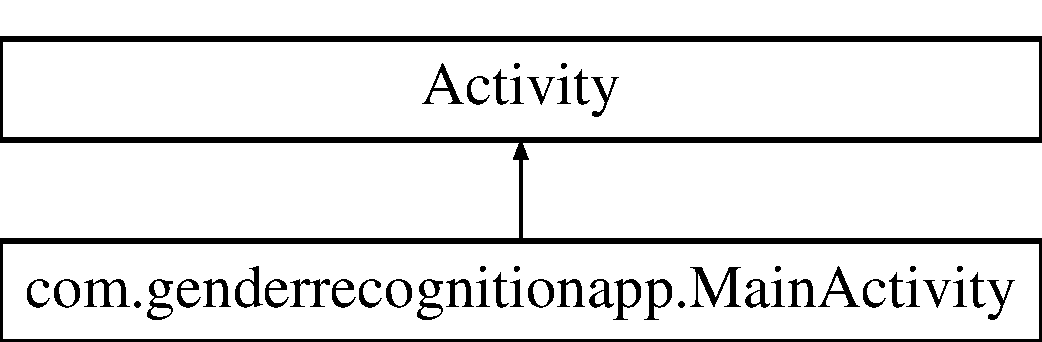
\includegraphics[height=2.000000cm]{classcom_1_1genderrecognitionapp_1_1_main_activity}
\end{center}
\end{figure}
\subsection*{Static Public Member Functions}
\begin{DoxyCompactItemize}
\item 
static void \hyperlink{classcom_1_1genderrecognitionapp_1_1_main_activity_ad6fe22aaba9d78c5bbfa4d61ae5aa6bd}{show\+Confirmation\+Pop\+Up} (String title, String text, int image)
\end{DoxyCompactItemize}
\subsection*{Static Public Attributes}
\begin{DoxyCompactItemize}
\item 
\hypertarget{classcom_1_1genderrecognitionapp_1_1_main_activity_a866fd5ba60bdb60bae99124ee88ada56}{}static Text\+View {\bfseries pitch\+Info}\label{classcom_1_1genderrecognitionapp_1_1_main_activity_a866fd5ba60bdb60bae99124ee88ada56}

\item 
\hypertarget{classcom_1_1genderrecognitionapp_1_1_main_activity_acc0c4c5ea9c43f38c0dbf17bd205083d}{}static Text\+View {\bfseries threshold\+Info}\label{classcom_1_1genderrecognitionapp_1_1_main_activity_acc0c4c5ea9c43f38c0dbf17bd205083d}

\item 
\hypertarget{classcom_1_1genderrecognitionapp_1_1_main_activity_a60bd4a7bf2a8b139097ce4ee8b151ea3}{}static Image\+View {\bfseries imageview}\label{classcom_1_1genderrecognitionapp_1_1_main_activity_a60bd4a7bf2a8b139097ce4ee8b151ea3}

\end{DoxyCompactItemize}
\subsection*{Protected Member Functions}
\begin{DoxyCompactItemize}
\item 
void \hyperlink{classcom_1_1genderrecognitionapp_1_1_main_activity_a624a983c43dfd05f56a72c8069491eaa}{on\+Create} (Bundle saved\+Instance\+State)
\end{DoxyCompactItemize}


\subsection{Member Function Documentation}
\hypertarget{classcom_1_1genderrecognitionapp_1_1_main_activity_a624a983c43dfd05f56a72c8069491eaa}{}\index{com\+::genderrecognitionapp\+::\+Main\+Activity@{com\+::genderrecognitionapp\+::\+Main\+Activity}!on\+Create@{on\+Create}}
\index{on\+Create@{on\+Create}!com\+::genderrecognitionapp\+::\+Main\+Activity@{com\+::genderrecognitionapp\+::\+Main\+Activity}}
\subsubsection[{on\+Create}]{\setlength{\rightskip}{0pt plus 5cm}void com.\+genderrecognitionapp.\+Main\+Activity.\+on\+Create (
\begin{DoxyParamCaption}
\item[{Bundle}]{saved\+Instance\+State}
\end{DoxyParamCaption}
)\hspace{0.3cm}{\ttfamily [protected]}}\label{classcom_1_1genderrecognitionapp_1_1_main_activity_a624a983c43dfd05f56a72c8069491eaa}
Retrieve a reference to an instance of Telephony\+Manager

\textquotesingle{}rec\textquotesingle{} object is executed with \textquotesingle{}rec.\+execute\textquotesingle{} with the same syntax we have seen used for the asynctask (as \textquotesingle{}rec\textquotesingle{} is). \hypertarget{classcom_1_1genderrecognitionapp_1_1_main_activity_ad6fe22aaba9d78c5bbfa4d61ae5aa6bd}{}\index{com\+::genderrecognitionapp\+::\+Main\+Activity@{com\+::genderrecognitionapp\+::\+Main\+Activity}!show\+Confirmation\+Pop\+Up@{show\+Confirmation\+Pop\+Up}}
\index{show\+Confirmation\+Pop\+Up@{show\+Confirmation\+Pop\+Up}!com\+::genderrecognitionapp\+::\+Main\+Activity@{com\+::genderrecognitionapp\+::\+Main\+Activity}}
\subsubsection[{show\+Confirmation\+Pop\+Up}]{\setlength{\rightskip}{0pt plus 5cm}static void com.\+genderrecognitionapp.\+Main\+Activity.\+show\+Confirmation\+Pop\+Up (
\begin{DoxyParamCaption}
\item[{String}]{title, }
\item[{String}]{text, }
\item[{int}]{image}
\end{DoxyParamCaption}
)\hspace{0.3cm}{\ttfamily [static]}}\label{classcom_1_1genderrecognitionapp_1_1_main_activity_ad6fe22aaba9d78c5bbfa4d61ae5aa6bd}
In order to link \textquotesingle{}custom\+\_\+dialog.\+xml\textquotesingle{} with the X\+M\+L Activity we have created this class and we have linked with \textquotesingle{}set\+Content\+View\textquotesingle{}. The differences between the previous code is that, here, we have to specify the related layout \textquotesingle{}confirmation\+Pop\+Up.\+find\+View\+By\+Id\textquotesingle{} by dot operator\+: this indicate that the image we are using is the \textquotesingle{}custom\+\_\+dialog.\+xml\textquotesingle{} one, defined in the initialization of the \textquotesingle{}confirmation\+Pop\+Up\textquotesingle{} object \mbox{[}Show confirmation of recording\mbox{]}\+: (\hyperlink{classcom_1_1genderrecognitionapp_1_1_main_activity_ad6fe22aaba9d78c5bbfa4d61ae5aa6bd}{show\+Confirmation\+Pop\+Up}) Set the dialog components

If button is clicked, close the custom dialog 

The documentation for this class was generated from the following file\+:\begin{DoxyCompactItemize}
\item 
src/com/genderrecognitionapp/Main\+Activity.\+java\end{DoxyCompactItemize}

\hypertarget{classcom_1_1example_1_1genderrecognitionapp_1_1_r}{}\section{com.\+example.\+genderrecognitionapp.\+R Class Reference}
\label{classcom_1_1example_1_1genderrecognitionapp_1_1_r}\index{com.\+example.\+genderrecognitionapp.\+R@{com.\+example.\+genderrecognitionapp.\+R}}
\subsection*{Classes}
\begin{DoxyCompactItemize}
\item 
class {\bfseries attr}
\item 
class {\bfseries drawable}
\item 
class {\bfseries id}
\item 
class {\bfseries layout}
\item 
class {\bfseries string}
\item 
class {\bfseries style}
\end{DoxyCompactItemize}


The documentation for this class was generated from the following file\+:\begin{DoxyCompactItemize}
\item 
gen/com/example/genderrecognitionapp/R.\+java\end{DoxyCompactItemize}

\hypertarget{classcom_1_1genderrecognitionapp_1_1_rec}{}\section{com.\+genderrecognitionapp.\+Rec Class Reference}
\label{classcom_1_1genderrecognitionapp_1_1_rec}\index{com.\+genderrecognitionapp.\+Rec@{com.\+genderrecognitionapp.\+Rec}}
Inheritance diagram for com.\+genderrecognitionapp.\+Rec\+:\begin{figure}[H]
\begin{center}
\leavevmode
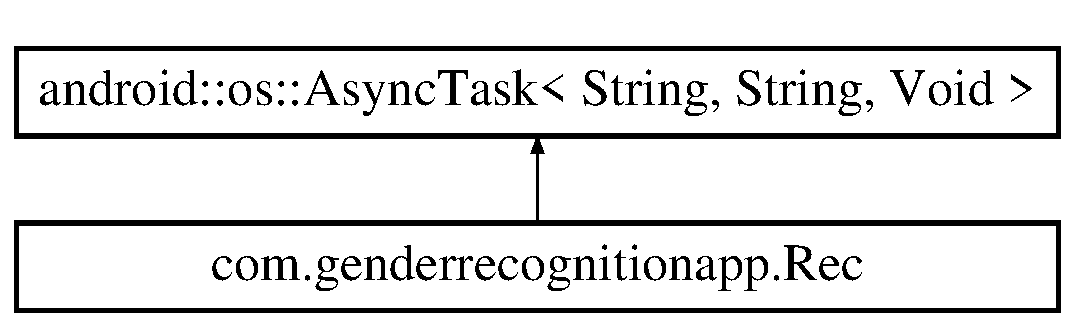
\includegraphics[height=2.000000cm]{classcom_1_1genderrecognitionapp_1_1_rec}
\end{center}
\end{figure}
\subsection*{Public Member Functions}
\begin{DoxyCompactItemize}
\item 
\hypertarget{classcom_1_1genderrecognitionapp_1_1_rec_a967ff86b9f93c1d26e5c109e488d2d4c}{}{\bfseries Rec} (Context context, int registration\+Lenght, int sample\+Frequency, short\mbox{[}$\,$\mbox{]} audio\+Data, short flag)\label{classcom_1_1genderrecognitionapp_1_1_rec_a967ff86b9f93c1d26e5c109e488d2d4c}

\end{DoxyCompactItemize}
\subsection*{Public Attributes}
\begin{DoxyCompactItemize}
\item 
\hypertarget{classcom_1_1genderrecognitionapp_1_1_rec_adf8991b349171c493924945cb29b17fb}{}short {\bfseries flag} = 0\label{classcom_1_1genderrecognitionapp_1_1_rec_adf8991b349171c493924945cb29b17fb}

\end{DoxyCompactItemize}
\subsection*{Protected Member Functions}
\begin{DoxyCompactItemize}
\item 
Void \hyperlink{classcom_1_1genderrecognitionapp_1_1_rec_a3bd30779d76fcc812c1a6bad9d22d265}{do\+In\+Background} (String...\+params)
\end{DoxyCompactItemize}
{\bf }\par
\begin{DoxyCompactItemize}
\item 
void \hyperlink{classcom_1_1genderrecognitionapp_1_1_rec_a6e3f7628a0219539f50e9995eec9daaa}{on\+Pre\+Execute} ()
\item 
\hypertarget{classcom_1_1genderrecognitionapp_1_1_rec_a1dd8d6b828c5173eebc33682ce981b5d}{}void {\bfseries on\+Post\+Execute} (Void \+\_\+v)\label{classcom_1_1genderrecognitionapp_1_1_rec_a1dd8d6b828c5173eebc33682ce981b5d}

\end{DoxyCompactItemize}



\subsection{Member Function Documentation}
\hypertarget{classcom_1_1genderrecognitionapp_1_1_rec_a3bd30779d76fcc812c1a6bad9d22d265}{}\index{com\+::genderrecognitionapp\+::\+Rec@{com\+::genderrecognitionapp\+::\+Rec}!do\+In\+Background@{do\+In\+Background}}
\index{do\+In\+Background@{do\+In\+Background}!com\+::genderrecognitionapp\+::\+Rec@{com\+::genderrecognitionapp\+::\+Rec}}
\subsubsection[{do\+In\+Background}]{\setlength{\rightskip}{0pt plus 5cm}Void com.\+genderrecognitionapp.\+Rec.\+do\+In\+Background (
\begin{DoxyParamCaption}
\item[{String...}]{params}
\end{DoxyParamCaption}
)\hspace{0.3cm}{\ttfamily [protected]}}\label{classcom_1_1genderrecognitionapp_1_1_rec_a3bd30779d76fcc812c1a6bad9d22d265}
In \textquotesingle{}params\mbox{[}\mbox{]}\textquotesingle{} will be stored value of path and filename that I have passed from the \textquotesingle{}\hyperlink{classcom_1_1genderrecognitionapp_1_1_main_activity}{Main\+Activity}\textquotesingle{} in the \textquotesingle{}execute\textquotesingle{} of the asynctask

\textquotesingle{}start\+Recording\textquotesingle{} � un A\+P\+I di Android

\textquotesingle{}0x00ff\textquotesingle{} is used to compute the A\+N\+Dlogic in binary logic and isolate 8 bit per time. If we would like to store in an other audio format we could be but implementing a different header\+: there is the problem about the signal processing behind other audio format (e.\+g. M\+P3), .W\+A\+V is not compressed

Entering in the \textquotesingle{}Wav\+I\+O\textquotesingle{} class in order to read documentation \hypertarget{classcom_1_1genderrecognitionapp_1_1_rec_a6e3f7628a0219539f50e9995eec9daaa}{}\index{com\+::genderrecognitionapp\+::\+Rec@{com\+::genderrecognitionapp\+::\+Rec}!on\+Pre\+Execute@{on\+Pre\+Execute}}
\index{on\+Pre\+Execute@{on\+Pre\+Execute}!com\+::genderrecognitionapp\+::\+Rec@{com\+::genderrecognitionapp\+::\+Rec}}
\subsubsection[{on\+Pre\+Execute}]{\setlength{\rightskip}{0pt plus 5cm}void com.\+genderrecognitionapp.\+Rec.\+on\+Pre\+Execute (
\begin{DoxyParamCaption}
{}
\end{DoxyParamCaption}
)\hspace{0.3cm}{\ttfamily [protected]}}\label{classcom_1_1genderrecognitionapp_1_1_rec_a6e3f7628a0219539f50e9995eec9daaa}
Object recorder in Android. \textquotesingle{}Media...M\+I\+C\textquotesingle{} is used to access in a static way to the integer that identify the micorphone \textquotesingle{}m\+Number\+Of\+Samples $\ast$ 2\textquotesingle{} is due to the fact that are \textquotesingle{}byte\textquotesingle{}, but we need to use \textquotesingle{}short\textquotesingle{} 

The documentation for this class was generated from the following file\+:\begin{DoxyCompactItemize}
\item 
src/com/genderrecognitionapp/Rec.\+java\end{DoxyCompactItemize}

\hypertarget{classcom_1_1wav_1_1_signal_processing}{}\section{com.\+wav.\+Signal\+Processing Class Reference}
\label{classcom_1_1wav_1_1_signal_processing}\index{com.\+wav.\+Signal\+Processing@{com.\+wav.\+Signal\+Processing}}
\subsection*{Public Member Functions}
\begin{DoxyCompactItemize}
\item 
\hypertarget{classcom_1_1wav_1_1_signal_processing_a45bbf5dd41837a2fffdd8e56a671467c}{}{\bfseries Signal\+Processing} (int\mbox{[}$\,$\mbox{]}\mbox{[}$\,$\mbox{]} frames)\label{classcom_1_1wav_1_1_signal_processing_a45bbf5dd41837a2fffdd8e56a671467c}

\item 
double\mbox{[}$\,$\mbox{]}\mbox{[}$\,$\mbox{]} \hyperlink{classcom_1_1wav_1_1_signal_processing_ab597d6a27eb6cddcaadb04f3c82a994e}{F\+F\+T} ()
\begin{DoxyCompactList}\small\item\em \mbox{[}F\+F\+T\mbox{]}\+: (\hyperlink{classcom_1_1wav_1_1_signal_processing_ab597d6a27eb6cddcaadb04f3c82a994e}{F\+F\+T}) \end{DoxyCompactList}\item 
double\mbox{[}$\,$\mbox{]}\mbox{[}$\,$\mbox{]} \hyperlink{classcom_1_1wav_1_1_signal_processing_a35bf021287fdbbab4f7f98b5363fb779}{compute\+Spectrum} (double\mbox{[}$\,$\mbox{]}\mbox{[}$\,$\mbox{]} fft\+Value\+Output)
\begin{DoxyCompactList}\small\item\em \mbox{[}Compute Spectrum\mbox{]}\+: (\hyperlink{classcom_1_1wav_1_1_signal_processing_a35bf021287fdbbab4f7f98b5363fb779}{compute\+Spectrum}) \end{DoxyCompactList}\item 
int\mbox{[}$\,$\mbox{]} \hyperlink{classcom_1_1wav_1_1_signal_processing_aa595ae30d87aeaedd07acbd5b9fd4d8c}{get\+Pitch\+Of\+Every\+Frames} (double\mbox{[}$\,$\mbox{]}\mbox{[}$\,$\mbox{]} spectrum)
\begin{DoxyCompactList}\small\item\em \mbox{[}Get Pitch of every frames\mbox{]}\+: (\hyperlink{classcom_1_1wav_1_1_signal_processing_aa595ae30d87aeaedd07acbd5b9fd4d8c}{get\+Pitch\+Of\+Every\+Frames}) \end{DoxyCompactList}\item 
int \hyperlink{classcom_1_1wav_1_1_signal_processing_ae35173b21b6e7994304fe7a5272d2c0e}{find\+Final\+Pitch} (int\mbox{[}$\,$\mbox{]} pitch\+Of\+Frames)
\begin{DoxyCompactList}\small\item\em \mbox{[}Find final pitch\mbox{]}\+: (\hyperlink{classcom_1_1wav_1_1_signal_processing_ae35173b21b6e7994304fe7a5272d2c0e}{find\+Final\+Pitch}) \end{DoxyCompactList}\end{DoxyCompactItemize}


\subsection{Member Function Documentation}
\hypertarget{classcom_1_1wav_1_1_signal_processing_a35bf021287fdbbab4f7f98b5363fb779}{}\index{com\+::wav\+::\+Signal\+Processing@{com\+::wav\+::\+Signal\+Processing}!compute\+Spectrum@{compute\+Spectrum}}
\index{compute\+Spectrum@{compute\+Spectrum}!com\+::wav\+::\+Signal\+Processing@{com\+::wav\+::\+Signal\+Processing}}
\subsubsection[{compute\+Spectrum}]{\setlength{\rightskip}{0pt plus 5cm}double \mbox{[}$\,$\mbox{]}\mbox{[}$\,$\mbox{]} com.\+wav.\+Signal\+Processing.\+compute\+Spectrum (
\begin{DoxyParamCaption}
\item[{doublefft\+Value\+Output}]{\mbox{[}$\,$\mbox{]}\mbox{[}$\,$\mbox{]}}
\end{DoxyParamCaption}
)}\label{classcom_1_1wav_1_1_signal_processing_a35bf021287fdbbab4f7f98b5363fb779}


\mbox{[}Compute Spectrum\mbox{]}\+: (\hyperlink{classcom_1_1wav_1_1_signal_processing_a35bf021287fdbbab4f7f98b5363fb779}{compute\+Spectrum}) 

Index (j+1)/2 -\/$>$ due to the fact we have any more real and image part \hypertarget{classcom_1_1wav_1_1_signal_processing_ab597d6a27eb6cddcaadb04f3c82a994e}{}\index{com\+::wav\+::\+Signal\+Processing@{com\+::wav\+::\+Signal\+Processing}!F\+F\+T@{F\+F\+T}}
\index{F\+F\+T@{F\+F\+T}!com\+::wav\+::\+Signal\+Processing@{com\+::wav\+::\+Signal\+Processing}}
\subsubsection[{F\+F\+T}]{\setlength{\rightskip}{0pt plus 5cm}double \mbox{[}$\,$\mbox{]}\mbox{[}$\,$\mbox{]} com.\+wav.\+Signal\+Processing.\+F\+F\+T (
\begin{DoxyParamCaption}
{}
\end{DoxyParamCaption}
)}\label{classcom_1_1wav_1_1_signal_processing_ab597d6a27eb6cddcaadb04f3c82a994e}


\mbox{[}F\+F\+T\mbox{]}\+: (\hyperlink{classcom_1_1wav_1_1_signal_processing_ab597d6a27eb6cddcaadb04f3c82a994e}{F\+F\+T}) 

Define compute the F\+F\+T and return matrix of value coupled in real and image part (because it\textquotesingle{}s a complex number!) Documentation of \textquotesingle{}F\+F\+T\textquotesingle{} algorithm\+: \{\href{https://sites.google.com/site/piotrwendykier/software/jtransforms}{\tt https\+://sites.\+google.\+com/site/piotrwendykier/software/jtransforms}\} Matrix which stores the n� of frames needed for the F\+F\+T computing for every frame. (The product for two is due to the complex exit of the F\+F\+T)

This is the array that, at first, contains the samples of the frame in time domain, after,the same samples but in the Fourier domain

Single frame

Compute F\+F\+T \hypertarget{classcom_1_1wav_1_1_signal_processing_ae35173b21b6e7994304fe7a5272d2c0e}{}\index{com\+::wav\+::\+Signal\+Processing@{com\+::wav\+::\+Signal\+Processing}!find\+Final\+Pitch@{find\+Final\+Pitch}}
\index{find\+Final\+Pitch@{find\+Final\+Pitch}!com\+::wav\+::\+Signal\+Processing@{com\+::wav\+::\+Signal\+Processing}}
\subsubsection[{find\+Final\+Pitch}]{\setlength{\rightskip}{0pt plus 5cm}int com.\+wav.\+Signal\+Processing.\+find\+Final\+Pitch (
\begin{DoxyParamCaption}
\item[{int\mbox{[}$\,$\mbox{]}}]{pitch\+Of\+Frames}
\end{DoxyParamCaption}
)}\label{classcom_1_1wav_1_1_signal_processing_ae35173b21b6e7994304fe7a5272d2c0e}


\mbox{[}Find final pitch\mbox{]}\+: (\hyperlink{classcom_1_1wav_1_1_signal_processing_ae35173b21b6e7994304fe7a5272d2c0e}{find\+Final\+Pitch}) 

This line compute the average of pitch frequency for every frame \hypertarget{classcom_1_1wav_1_1_signal_processing_aa595ae30d87aeaedd07acbd5b9fd4d8c}{}\index{com\+::wav\+::\+Signal\+Processing@{com\+::wav\+::\+Signal\+Processing}!get\+Pitch\+Of\+Every\+Frames@{get\+Pitch\+Of\+Every\+Frames}}
\index{get\+Pitch\+Of\+Every\+Frames@{get\+Pitch\+Of\+Every\+Frames}!com\+::wav\+::\+Signal\+Processing@{com\+::wav\+::\+Signal\+Processing}}
\subsubsection[{get\+Pitch\+Of\+Every\+Frames}]{\setlength{\rightskip}{0pt plus 5cm}int \mbox{[}$\,$\mbox{]} com.\+wav.\+Signal\+Processing.\+get\+Pitch\+Of\+Every\+Frames (
\begin{DoxyParamCaption}
\item[{double}]{spectrum\mbox{[}$\,$\mbox{]}\mbox{[}$\,$\mbox{]}}
\end{DoxyParamCaption}
)}\label{classcom_1_1wav_1_1_signal_processing_aa595ae30d87aeaedd07acbd5b9fd4d8c}


\mbox{[}Get Pitch of every frames\mbox{]}\+: (\hyperlink{classcom_1_1wav_1_1_signal_processing_aa595ae30d87aeaedd07acbd5b9fd4d8c}{get\+Pitch\+Of\+Every\+Frames}) 

\textquotesingle{}frequency\+Step\textquotesingle{} represents the frequency gap between the samples

This block finds the index related to the maximum value of amplitude of the spectrum for every frame

Links the frequency with the right sample 

The documentation for this class was generated from the following file\+:\begin{DoxyCompactItemize}
\item 
src/com/wav/Signal\+Processing.\+java\end{DoxyCompactItemize}

\hypertarget{classcom_1_1wav_1_1_wav_i_o}{}\section{com.\+wav.\+Wav\+I\+O Class Reference}
\label{classcom_1_1wav_1_1_wav_i_o}\index{com.\+wav.\+Wav\+I\+O@{com.\+wav.\+Wav\+I\+O}}
\subsection*{Public Member Functions}
\begin{DoxyCompactItemize}
\item 
\hypertarget{classcom_1_1wav_1_1_wav_i_o_af9f6dce5f7ade899a5edfe052e7deed6}{}String {\bfseries get\+Path} ()\label{classcom_1_1wav_1_1_wav_i_o_af9f6dce5f7ade899a5edfe052e7deed6}

\item 
\hypertarget{classcom_1_1wav_1_1_wav_i_o_a24c8926b5cbed9310f8f495b3991c41c}{}void {\bfseries set\+Path} (String new\+Path)\label{classcom_1_1wav_1_1_wav_i_o_a24c8926b5cbed9310f8f495b3991c41c}

\item 
\hypertarget{classcom_1_1wav_1_1_wav_i_o_a7ae7b501f83116930ff3b23a3708d739}{}{\bfseries Wav\+I\+O} (String tmp\+Path)\label{classcom_1_1wav_1_1_wav_i_o_a7ae7b501f83116930ff3b23a3708d739}

\item 
\hypertarget{classcom_1_1wav_1_1_wav_i_o_a843f42f2c686bb4442717ff31da303c4}{}{\bfseries Wav\+I\+O} (String tmp\+Path, long sub\+Chunk1\+Size, int format, long channels, long sample\+Rate, int block\+Align, int bits\+Per\+Sample, byte\mbox{[}$\,$\mbox{]} audio\+Data)\label{classcom_1_1wav_1_1_wav_i_o_a843f42f2c686bb4442717ff31da303c4}

\item 
\hypertarget{classcom_1_1wav_1_1_wav_i_o_a558cfecbda54ddc616bedad88a6835dc}{}boolean {\bfseries read} ()\label{classcom_1_1wav_1_1_wav_i_o_a558cfecbda54ddc616bedad88a6835dc}

\item 
\hypertarget{classcom_1_1wav_1_1_wav_i_o_a828ee12a5f9aaa5b1ab67f62be96b2f1}{}boolean {\bfseries save} ()\label{classcom_1_1wav_1_1_wav_i_o_a828ee12a5f9aaa5b1ab67f62be96b2f1}

\item 
\hypertarget{classcom_1_1wav_1_1_wav_i_o_aa8a514d3d3da993f00dac0080d4c64bf}{}String {\bfseries get\+Summary} ()\label{classcom_1_1wav_1_1_wav_i_o_aa8a514d3d3da993f00dac0080d4c64bf}

\end{DoxyCompactItemize}
\subsection*{Static Public Member Functions}
\begin{DoxyCompactItemize}
\item 
\hypertarget{classcom_1_1wav_1_1_wav_i_o_aa6906f9503ee02b7f9722f635d2cb581}{}static int {\bfseries byte\+Array\+To\+Int} (byte\mbox{[}$\,$\mbox{]} b)\label{classcom_1_1wav_1_1_wav_i_o_aa6906f9503ee02b7f9722f635d2cb581}

\item 
\hypertarget{classcom_1_1wav_1_1_wav_i_o_a4abccfbfe2c9d49da330bc21c5c0272f}{}static long {\bfseries byte\+Array\+To\+Long} (byte\mbox{[}$\,$\mbox{]} b)\label{classcom_1_1wav_1_1_wav_i_o_a4abccfbfe2c9d49da330bc21c5c0272f}

\item 
\hypertarget{classcom_1_1wav_1_1_wav_i_o_a8dcd8c2ff6c82b006630950817c38b71}{}static byte\mbox{[}$\,$\mbox{]} {\bfseries short\+To\+Byte\+Array} (short data)\label{classcom_1_1wav_1_1_wav_i_o_a8dcd8c2ff6c82b006630950817c38b71}

\end{DoxyCompactItemize}
\subsection*{Public Attributes}
\begin{DoxyCompactItemize}
\item 
\hypertarget{classcom_1_1wav_1_1_wav_i_o_a6fb9e5ff2853a8fd3e244ce5a77b258e}{}byte\mbox{[}$\,$\mbox{]} {\bfseries my\+Data}\label{classcom_1_1wav_1_1_wav_i_o_a6fb9e5ff2853a8fd3e244ce5a77b258e}

\end{DoxyCompactItemize}


The documentation for this class was generated from the following file\+:\begin{DoxyCompactItemize}
\item 
src/com/wav/Wav\+I\+O.\+java\end{DoxyCompactItemize}

%--- End generated contents ---

% Index
\backmatter
\newpage
\phantomsection
\clearemptydoublepage
\addcontentsline{toc}{chapter}{Index}
\printindex

\end{document}
